%        File: notes.tex
%     Created: Tue Dec 01 09:00 PM 2015 G
% Last Change: Tue Dec 01 09:00 PM 2015 G
%
\documentclass[a4paper]{article}
\usepackage[margin=1in]{geometry}
\usepackage{amsmath}
\usepackage{amssymb,tabu}
\usepackage{array}
\usepackage{bm}
\usepackage{float}
\usepackage{enumerate}% http://ctan.org/pkg/enumerate
\usepackage{amsthm}
\newtheorem{theorem}{Theorem}
\usepackage{graphicx}
\usepackage{hyperref}
\hypersetup{
  colorlinks,
  citecolor=black,
  filecolor=black,
  linkcolor=black,
  urlcolor=black
}
\usepackage{tikz} 

\theoremstyle{definition} \newtheorem*{definition}{Definition}
\newtheorem{lemma}[theorem]{Lemma}
\newtheorem{proposition}[theorem]{Proposition}
\newtheorem*{corollary}{Corollary} \newtheorem*{remark}{Remark}
\newtheorem*{exmp}{Example} \newtheorem*{exmps}{Examples}
\newtheorem*{obvs}{Observation}
\newcommand{\naturals}{\mathbb{N}} 
\newcommand{\complexes}{\mathbb{C}}
\newcommand{\integers}{\mathbb{Z}}
\newcommand{\ent}{\bm{H}}
\newcommand{\pr}{\bm{p}}
\newcommand{\B}{\mathbb{B}}
\begin{document}
\title{Information and Codes}
\author{Michael Akintunde}
\maketitle

\section{Information}
\subsection{Coding and Decoding}
\begin{definition}
  The \emph{Entropy} of a probability distribution $p$ is
  \[
    H(p) = - \sum p(x)\log_2(p(x))
  \]
\end{definition}
\begin{exmp}
  Consider a Cheltenham Horse Race with 8 horses with winning chances
  \[
    p = \left(
    \frac{1}{2},\frac{1}{4},\frac{1}{8},\frac{1}{16},\frac{1}{64},
    \frac{1}{64},\frac{1}{64},\frac{1}{64}\right).
  \] 
  The entropy is therefore $-\left( \frac{1}{2}(-1) + \frac{1}{4}(-2) +
  \frac{1}{8} (-3) + \frac{1}{16} (-4) + \frac{1}{64}(-6)(4) \right) = 2$.
\end{exmp}

\begin{definition}
  An \emph{alphabet} is a finite set $S$; its members $s \in S$ are referred to
  as \emph{symbols}.
\end{definition}

\begin{definition}
  A \emph{message} $m$ in the alphabet $S$ is a finite sequence of 
  elements in $S$.
  \[
    m = s_1 s_2 \dots s_n \quad \text{with } s_i \in S,\,1 \leq i \leq n.
  \]

  A message is often also referred to as a \emph{string} or \emph{word}
  in $S$. The number $n \in \naturals$ is the \emph{length} of $m$.
\end{definition}

\begin{remark} We denote:
  \begin{itemize}
    \item 
      $|m| = n$.
    \item $m|_k = s_1s_2 \dots s_k$ (with $k \leq n$).
    \item $\varepsilon=$ The string of length zero, with $|\varepsilon| =
      0$.
    \item $S^0=$ Set of all words containing only $\varepsilon$.
    \item $S^n=$ Set of all strings of length $n$
    \item $S^*= S^0 \cup S^1 \cup S^2 \cup \dots$
  \end{itemize}
\end{remark}

\subsection{Coding}
\begin{definition}
  Let $S$ and $T$ be two alphabets. A \emph{code} is an \emph{injective}
  function 
  \[
    c : S \rightarrow T^*
  \]

  For each symbol $s \in S$ the string $c(s) \in T^*$ is called the 
  codeword for $s$. The set of all codewords
  \[
    C = \left\{ c(s) : s \in S \right\}
  \]
  Is also referred to as the code.
\end{definition}

\begin{remark}
  For $|T|=b$, we have a $b$-ary code.
\end{remark}

\begin{definition}
  A code $c : S \rightarrow T^*$ is extended to  $S^*$ as follows: Given
  a string $s_1s_2 \dots s_n \in S^*$ we define
  \[
    c(s_1s_2 \dots s_n) = c(s_1)c(s_2)\dots c(s_n)
  \]
\end{definition}

\begin{definition}
  A code $c : S \rightarrow T^*$ is \emph{uniquely decodeable} (UD) if the
  extended code function $c : S^{*} \rightarrow T^*$ is \emph{injective}.
  In other words, every string in $T^*$ corresponds to \emph{at most one} 
  message in $S^*$.
\end{definition}

\begin{definition}
  A code $c : S \rightarrow T^*$ is \emph{prefix-free} (short PF) if there
  is no pair of codewords $q = c(s)$ and $q' = c(s')$ such that

  \[
    q' = qr  \quad \text{for some non-empty word } r \in T^*
  \]

\end{definition}

\begin{theorem}
    If a code $c : S \rightarrow T^*$ is prefix-free then it is uniquely decodable.
    \label{thm:pfimpliesud}
\end{theorem}

\begin{proof}
  Take $x = x_1 x_2 \dots x_m$ and $y = y_1 y_2 \dots y_n$ such that $c(x)=c(y)$
  with $c(x)=c(x_1)c(x_2)\dots c(x_m)$ and $c(y)=c(y_1)c(y_2)\dots c(y_n)$.
  
  The prefixes (of length $k$)  must be the same $c(x)|_k = c(y)|_k$ for any $k$.
  It might be that $|c(x_1)|\neq |c(y_1)|$.

  Assume w.l.o.g $|c(x_1)| \leq |c(y_1)|$, and take $k = |c(x_1)|$ then 
  $c(x)|_k = c(x_1) = c(y_1)|_k$ and thus $c(y_1)=c(x_1)r$ for some $r \in T^*$.
  This contradicts PF. Repeat argument to cover all of $c(x)=c(y)$. Formally:
  induction on lengths $m$ and $n$.
\end{proof}

\begin{remark}
  The codewords in $C$ can be represented by the end-points of the 
  corresponding paths. If a code $C$ is PF then none of its descendents
  can represent a codeword in $C$.
\end{remark}

\begin{exmp}
  For the PF code $\left\{ 0,10,110,111 \right\}$, we have:
  \begin{figure}[!h]
    \centering
    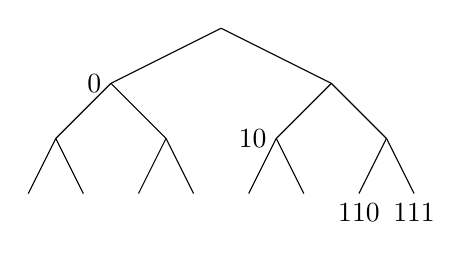
\begin{tikzpicture}[scale=0.7]
      \draw (0,0) -- (-2,-1);
      \draw (0,0) -- (2,-1);
      \draw (-2,-1) -- (-3,-2);
      \draw (-2,-1) -- (-1,-2);
      \node[left] at (-2,-1) {0};
      \draw (2,-1) -- (1, -2);
      \draw (2,-1) -- (3, -2);
      \draw (-3,-2) -- (-3.5, -3);
      \draw (-3,-2) -- (-2.5, -3);
      \draw (-1,-2) -- (-1.5, -3);
      \draw (-1,-2) -- (-0.5, -3);
      \draw (1, -2) -- (0.5, -3);
      \draw (1, -2) -- (1.5, -3);
      \node[left] at (1,-2) {10};
      \draw (3, -2) -- (2.5, -3);
      \node[below] at (2.5, -3) {110};
      \draw (3, -2) -- (3.5, -3);
      \node[below] at  (3.5, -3) {111};
    \end{tikzpicture}
    \caption{The corresponding tree for $C$.}
    \label{fig:treepf}
  \end{figure}
\end{exmp}

\begin{definition}
  Given a code $c : S \rightarrow T^*$, let $n_i$ denote the number of
  symbols $s \in S$ which are decoded by strings of length $i$, i.e.
  \[
    n_i = \Big| \left\{ s \in S : |c(s)| = i \right\} \Big| = 
  \Big| \left\{( s \in S : c(s) \in T^i \right\} \Big|
  \]

  We refer to $n_1,n_2\dots n_M$ as \emph{parameters} of $c$, where
  $M$ is the \emph{maximal length} of a codeword.
\end{definition}

\begin{remark}
  We denote:
\begin{itemize}
  \item $b^i=|T^i|$: The number of all potential codewords of length $i$.
  \item $\frac{n_i}{b^i}$: The fraction of possible codewords of length
    $i$ which is actually used by a code.
\end{itemize}
\end{remark}

\begin{definition}
  Given a code $c:S \rightarrow T^*$ with parametrs $n_1,n_2,\dots, n_M$. 
  The Kraft-McMillan Number of $c$ is defined as:
  \[
    K = \sum_{i=1}^M \frac{n_i}{b^i} = \frac{n_1}{b} + \frac{n_2}{b^2} +
    \dots + \frac{n_M}{b^M}
  \]
\end{definition}

\begin{theorem}
  (L.G. Kraft, 1949). Given an alphabet $T$ with $|T| = b$ and (code)
  parameters $n_1, n_2, \dots, n_M \in \naturals$. 
  
  If $K \leq 1$ there
  exists a PF $b-$ary code $c:S \rightarrow T^*$ with these parameters.
  \label{thm:lgkraft}
\end{theorem}

\begin{remark}
  We denote $q_r(i) = \Big| \left\{ |c(s)|=i : |s| = r \right\} \Big|$.
  (The number of strings of length $r$ encoded
  in a string of length $i$).
\end{remark}

\begin{definition}
  For a sequence of numbers $q(1), q(2), q(3)\dots$ the \emph{generating function} $Q(x)$ is given as the polynomial (formal power series) in the 
  unknown variable $x$:
  \[
    Q(x) = q(1)x + q(2)x^2 + q(3)x^3 + \dots
  \]
\end{definition}

\begin{remark}
  For a code $c:S \rightarrow T^*$ we have for $1 \leq i \leq rM$:
  \[
    Q_r(x) = \sum_{i=1}^{rM} q_r(i)x^i =  q_r(1)x + q_r(2)x^2 + \dots + q_r(rM)x^{rM}
  \]
\end{remark}

\begin{theorem}(Counting Principle).
  Given a UD code $s:S \rightarrow T^*$ with $|c(s)| \leq M$ for all
  $s \in S$ with generating function $Q_r(x)$ then for all $r \geq 1$:
  \[
    Q_r(x) = Q_1(x).
  \]
  \label{conutingprinciple}
\end{theorem}

\begin{theorem}
  (B. McMillan, 1956). If there exists a UD code $c :S \rightarrow T^*$
  with parameters $n_1,n_2, \dots, n_M \in \naturals$ then $K\leq 1$.
  \label{bmcmillan}
\end{theorem}

\begin{corollary}
  The following are equivalent:
  \begin{itemize}
    \item There exists a UD code with parameters $n_1, n_2, \dots, n_M$.
    \item It holds that $K \leq 1$ for parameters $n_1,n_2, \dots, n_M$.
    \item There exists a PF code with parameters $n_1,n_2, \dots, n_M$.
  \end{itemize}
\end{corollary}

\subsection{Representation of Information}
\begin{definition}
  Let $S$ be an alphabet. A source $(S,p)$ with probability distributions
  $p^{(k)} = \left( p_1^{(k)}, p_2^{(k)}, \dots , p_n^{(k)} \right)$ emits
  a stream (sequence) $\sigma_1\sigma_2\sigma_3 \dots$ of symbols with
  probability
  \[
    Pr(\sigma_k = s_i) = p_i^{(k)}.
  \]
\end{definition}
\begin{definition}
  Let $S$ be an alphabet. A \emph{memoryless} source $(S,p)$ emits
  a stream (sequence) $\sigma_1\sigma_2\sigma_3 \dots$ 
  such that for all $k$ and $l$:
  \[
    Pr(\sigma_k = s_i \land \sigma_l = s_j) = Pr(\sigma_k =
    s_i)Pr(\sigma_l = s_j).
  \]
\end{definition}

\begin{definition}
  A (discrete time) \emph{stochastic process} on a (state) space $S$ is
  a collection of $S-$ valued random variables $X_i$ with $i \in
  \naturals$ or $\integers$. Then:

  \begin{align*}
    Pr(X_0 &= s_{i_0} \land X_1 = s_{i_1} \land \dots 
    \land X_N = s_{i_N}) = \\
    &P(X_0 = s_{i_0}) \cdot \\
     &Pr( X_1 = s_{i_1} | X_0 = s_{i_0}) \cdot \cdots \\
     &Pr(X_N = s_{i_N} | X_0 = s_{i_0} \land X_1 = s_{i_1} \dots \land
    X_{N-1} = s_{i_{N-1}})
  \end{align*}
\end{definition}

\begin{definition}
  A (discrete time) \emph{Markov Chain} is a stochastic process with
  $\forall N$
  \begin{align*}
    Pr(X_N &= s_{i_N} | X_0 = s_{i_0} \land X_1 = s_{i_1} \dots \land
        X_{N-1} = s_{i_{N-1}}) = \\
        &Pr(X_N = s_{i_N} | X_{N-1} = s_{i_{N-1}})
  \end{align*}

  A DTMC can be specified by a \emph{stochastic} square matrix
  \[
    \boxed{(P_{ij}) = Pr(X_N = s_i | X_{N-1} = s_j)} \quad \text{with } 
    \sum_{s_i \in S} P_{ij} = 1
  \]
\end{definition}

\begin{remark}
  \hfill
  \begin{itemize}
    \item Remember \emph{Nothing}: Memoryless Process.
    \item Remember \emph{Last State}: Markov Chain.
    \item Remember \emph{Everything}: Stochastic Process.
  \end{itemize}
\end{remark}

\begin{definition}
  The \emph{average word length} $L$ of a code $c : S \rightarrow T^*$ for
  a source $(S,p)$ is 
  \[
    \boxed{L = p_1l_1 + p_2l_2 + \dots p_ml_m = \sum_{i=1}^m p_il_i = E(l).}
  \]
  with $l_i = |c(s_i)|$ being the length of codewords in $T^*$ for each
  $s_i \in S$.
\end{definition}

\begin{definition}
  (Optimal code). Given a source $(S, p)$ and an alphabet $T$, a 
  UD code $c:S \rightarrow T^*$ is \emph{optimal} if there is no other 
  code $c' : S \rightarrow T^*$ with smaller average word length.
\end{definition}

\begin{definition}
  (Entropy of a distribution). Given a distribution $p = (p_1, p_2, \dots,
  p_m)$, the \emph{entropy} of $p$ (of base $b$) is given by
  \[
    \boxed{  H_b(p) = \sum_{i=1}^m p_i \log_b \left( \frac{1}{p_i} \right).}
  \]
\end{definition}

\begin{theorem}
  (Comparision Theorem). Given probability distributions $p = 
  \left( p_1, p_2, \dots , p_m \right)$ and $q = \left( q_1, q_2, \dots
  , q_m\right)$, then
  \[
   \boxed{ H_b(p) = \sum_{i=1}^m p_i \cdot \log_b\left( \frac{1}{p_i} \right)
   \leq \sum_{i=1}^m p_i \cdot\log_b\left( \frac{1}{q_i} \right)}
  \]
  \label{thm:comparison}
  Equality holds iff $p_i = q_i$ for all $1 \leq i \leq m$.
\end{theorem}

\begin{theorem}
  The entropy of a probability distribution $p$ on $m$ symbols is at most
  $\log_b(m)$, i.e. 
  \[
    \boxed{ H_b(p) \leq \log_b(m).}
  \]
  There is equality iff $p_i = \frac{1}{m}$ for all symbols.
  \label{thm:uniform}
\end{theorem}

\begin{theorem}
  (Fundamental Theorem). The average word length of any UD code 
  $c : S \rightarrow T^*$ with $|T|=b$ for the source $(S,p)$ satisfies
  \[
    \boxed{L \geq H_b(p)}
  \]
  \label{thm:fundamental}
\end{theorem}

\subsubsection*{Shannon-Fano Rule}
\begin{definition}
  (Shannon-Fano Rule). Select the word length for symbol $s_i$ the least
  possibl integer such that $b^{y_i}\geq \frac{1}{p_i}$
\end{definition}

\begin{theorem}
  There exists a prefix-free code $c:S \rightarrow T^*$ with $|T|=b$ for the
  source $(S,\bm{p})$ which satisfies $L < \bm{H}_b(\bm{p})+1$.
  \label{SF}
\end{theorem}

\subsubsection*{Optimal PF Codes}
\begin{lemma}
  For an optimal prefix-free code $c:S \rightarrow \B^*$ for a source
  $(S,\pr)$:
  \begin{itemize}
    \item $|c(s')| > |c(s)| \implies p_s \geq p_s'$
    \item Among the codewords of maximal length there are two of the form
      $w0$ and $w1$ for some $w \in \B^{*}$.
  \end{itemize}
  \label{optpf}
\end{lemma}

\subsubsection*{Huffman's Rule}
Huffman's Rule is used to construct \emph{optimal codes}.
\begin{enumerate}
  \item Given a source $(S,\pr)$, let $s'$ and $s''$ be symbols with 
    smallest probability. Construct $(S^*,\pr^*)$ by replacing $s'$ and
    $s''$ with a new symbol $s^*$ with probability 
    $p_{s^*}=p_{s'}+p_{s''}$
  \item Given a PF binary code $h^*$ for $(S,\pr)$ with 
    $h^*:s^*\mapsto w$ then define a binary code $h$ for $(S,\pr)$ with
    $h:s' \mapsto w0$ and $h : s'' \mapsto w1$.
\end{enumerate}

\begin{lemma}
  Let codes $h$ and $h^*$ be defined as required by H2. Then the average
  word legthsof $h$ and $h'$ satisfy:
  \[
    L(h)=L(h^*)+p_*^*
  \]
  \label{avgwordlength}
\end{lemma}

\begin{theorem}
  (Optimality of Huffman Code). 
  If code $h'$ is optimal for $(S^*,p^*)$ then code $h$ is optimal for
  $(S,p).$
  \label{optimalhuff}
\end{theorem}
\end{document}


